\section{Einführung}
\label{sec:einfuehrung}
% \IEEEPARstart{H}{eutzutage} gibt es zu viele Probleme
% Today, many organizations deploy a multitude of services on a large
% number of servers. In some cases, all these services run on different
% machines not because one machine cannot handle the load, but for
% reasons of reliability.  All software is faulty~\cite{zellerprograms},
% and operating systems with thousands of lines of code, running servers
% written by different software vendors simply cannot be trusted to
% provide uptimes of 99.9 percent or more. Putting each service on a
% separate machine will achieve reliability at the expense of
% maintainability simply because a large number of physical machines is
% involved.

% Virtual machine technology has been around for more than 40
% years~\cite{tanenbaum1992modern}. The technology to host multiple
% machines on a single system reduces the space and power requirements
% for data centers and represents enormous cost savings for companies
% like Amazon, Microsoft or Google, which deploy hundreds or thousands
% of servers for a variety of services. Unsurprisingly, virtualization
% for cost reduction and transparent scalability is becoming
% increasingly popular. Cloud providers such as Amazon, Rackspace or
% Engine Yard offer scalable hosting solutions for companies and
% individuals who cannot of do not want to maintain a private cloud.

% There are obvious issues with isolation, however. As a service
% provider, I want to avoid downtime as much as possible. Thus, I cannot
% easily move my virtual machine from one provider to another. I cannot
% easily migrate existing VMs to new a hypervisor architecture or a
% completely new virtualization solution. If hardware is failing, I
% cannot simply migrate the VM to new hardware without taking it down.

% Asger Jensen and Dr. Jacob Gorm Hansen proposed live VM migration as a
% solution to these problems. They were the first to demonstrate live
% migration of a running VM in 2002 on a research hypervisor called
% NomadBIOS. 
- Firmen sehen heutzutage so aus
- Cloud könnte für sie interessant sein
- Welche Rolle Live-Migration da für sie spielt, und wie es ihnen
helfen kann, zeigen wir

\subsection{Der Status in Rechenzentren}
- Derzeit Rechner im Rechenzentrum
- Cluster
- Grid
- Probleme:
  - Ungleichmäßige Auslastung
  - Wartungskosten (Admins)
  - Downtime bei Upgrades/HW-Problemen
  - Operationskosten (Strom)

\subsection{Die Cloud als Ziel}
\label{sec:sota}
- Public vs Private
Für potentielle Nutzer einer Cloud Lösung präsentieren sich derzeit
zwei Möglichkeiten: Eine eigene, business-interne Cloud Plattform zu
installieren, oder 

In this part we will explore the state of the art in live VM
migration, both from a technical as from a use-case point of view.
Ich will scalieren:
\begin{itemize}
\item Public Cloud
\item Private Cloud
\end{itemize}
- Um zu entscheiden zunächst wissen, {\bf was} in die cloud geht

\subsubsection{Level der Virtualisierung}
\label{sec:def-virtualisierung}

\begin{figure*}[htbp]
  \centering
  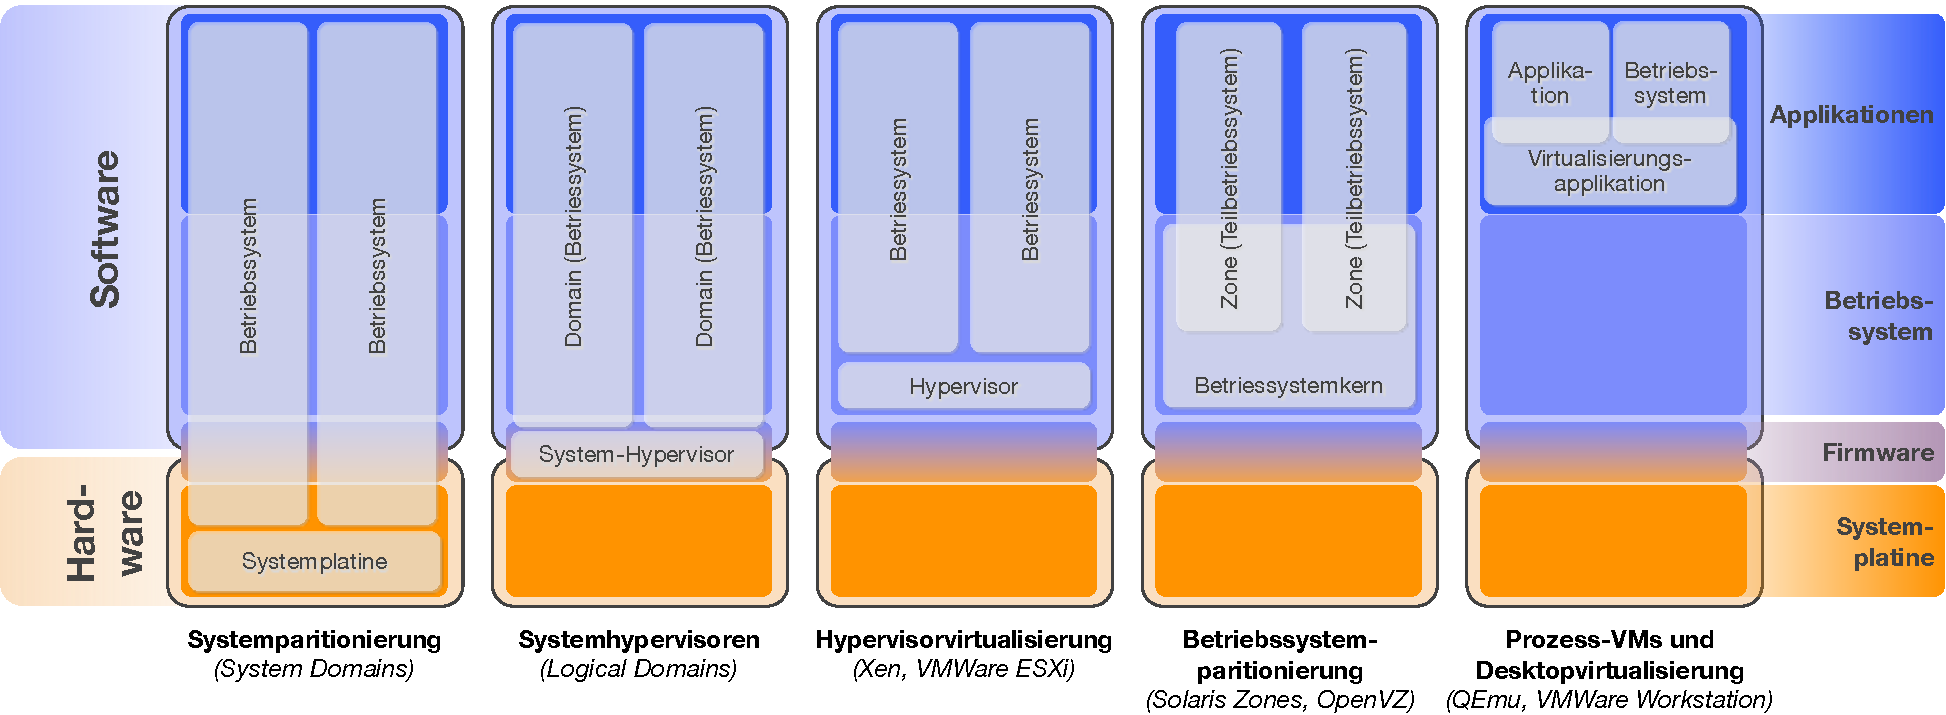
\includegraphics[width=\textwidth]{images/Virtualisierungslevel}
  \caption{Virtualisierung kann auf verschiedenen Ebenen angesetzt werden. Im Kontext von Live-Migration sind die vertikal eingezeichneten Elemente, das heißt, die zu virtualisierenden Betriebssysteme oder Applikationen von Interesse. }
  \label{fig:levels}
\end{figure*}

Virtualisierung kann auf verschiedenen Ebenen stattfinden. Je näher an
der Hardware die Virtualisierung stattfindet, desto mehr kann die
Hardware auch unterstützend wirken. Je ferner der Hardware, desto
weniger ist die Virtualisierung von der unterliegenden Hardware
abhängig.~\cite{Giesekus2010:Virtualisierung} In diesem Zusammenhang
beschreiben \emph{Konsolidierung} (insb. Server-Konsolidierung),
\emph{Separation} und \emph{Virtualisierung} verschiedene Perspektiven
auf den selben Sachverhalt: \emph{Das Nebeneinanderbetreiben von
Ausführungsumgebungen auf ein und derselben physischen Recheneinheit
ohne (oder mit minimaler) gegenseitige(r) Kenntnis.}

In der untersten Schicht kann die so genannte
\emph{Systempartitionierung} betrachtet werden (Siehe zu den Ebenen
\autoref{fig:levels}). Die "`Sun Fire Dynamic System
Domains"'~\cite{Shoumack2007:Beginners-Guid-}, die auf Sun Fire
Servern zur Verfügung steht, ist ein Beispiel für diesen
Virtualisierungsansatz. Die Hardware dieser Server ist in der Lage,
verschiedene Ausführungsumgebungen, das heißt, Betriebssysteme,
elektronisch isoliert zu betreiben. Es bedarf keinerlei Unterstützung
in den darüberliegenen Frimware- oder Softwareschichten. Diese Art
Virtualisierung kommt der Ausführung auf physikalisch getrennten
Rechnern am nächsten.

Eine Ebene höher kann Virtualisierung mit Hilfe von
\emph{Hypervisoren} betrieben werden. \acfp{VM} laufen auf
physikalischen Maschinen durch einen \emph{Hypervisor}, ein minimales
Betriebssystem, dass den Zugriff auf die physikalische Hardware regelt
und Routing zwischen dem physikalischen und virtuellen Netzwerk
bereitstellt~\cite{tanenbaum1992modern}. Wenn eine \ac{VM} ausfällt,
bleiben die anderen davon unbeeinflusst. Da des weiteren alle
Operationen innerhalb einer \ac{VM} virtualisiert sind, kann der Hypervisor
den Zustand eines virtuellen Servers in regelmäßigen Abständen
sichern, und so bei Ausfall die \ac{VM} von einer früheren Sicherung
wiederherstellen.

Ein Speziallfall der Virtualisierung mit Hypervisoren sind die
\emph{\acfp{ldom}}, die auf Rechnern mit Prozessoren der SPARC T-Serie
zur Verfügung stehen und unter dem Namen "`Oracle VM Server for
SPARC"'~\cite{Corporation:Oracle-VM-Serve} von Oracle vermarktet
werden. Dabei können die Ressourcen des Rechners in logische Bereiche
(\aclp{ldom}) eingeteilt werden, die gleichzeitig jeweils ein
Betriebssystem zur Verfügung stellen können. Damit ist es möglich,
ohne direkte Software-Unterstützung eine virtualisierte Ausführung
von Betriebssystemen zu haben: die Firmware der SPARC-Rechner stellt
Überwachungs- und Steuerungsfunktionalität bereit, die Hypervisoren
nicht unähnlich ist.

Auf Betriebssystemebene ist ebenfalls eine Art Virtualisierung
möglich. Dabei ist das Ziel, mehrere Exemplare der selben
Betriebssysteminstallation auszuführen. Ein Beispiel für diese
\emph{Betriebssystempartitionierung} (auch \emph{Servervirtualisierung
  auf Betriebssystemebene}) sind die "`Solaris
Zones"'~\cite{price2004solaris}. Sie erlauben, eine
Solaris-Installation mehrfach ausführen zu lassen, und zu einem
gewissen, einstellbaren Grad die installierten
Betriebssystemkomponenten nachzunutzen respektive zu ersetzen. Dabei
wird der Betriebssystemkern einmal ausgeführt, trägt aber Sorge dafür,
den einzelnen Zonen als "`ihr"' Kern zu erscheinen. Eine vergleichbare
Technologie für Linux-Systeme ist das
OpenVZ-Projekt~\cite{ahmed2008server}.

Auf Applikationsebene gibt es zwei unterschiedliche
Virtualisierungsansätze. Während \emph{Desktopvirtualisierung},
vergleichbar zur Hypervisorvirtualisierung, Betriebssysteme
virtualisiert und somit innerhalb eines anderen Betriebssystem bereit
stellt, haben Prozess-\acp{VM} das Ziel, eine Ausführungsumgebung für
bestimmte Programmiersprachen oder Applikationen bereit zu stellen.
Beispiele für ersteres sind VMWare
Workstation~\cite{VMWare-Inc:VMware-Workstat} oder Oracle
VirtualBox~\cite{Oracle-Corporation:VirtualBox} (vormals Sun xVM), für
letzteres \acp{VM} wie die
JVM~\cite{Sun-Developer-Network2003:The-Java-Virtua} oder
Smalltalk-Implementierungen~\cite{ansiSmalltalk}.

\subsubsection{Was geht in die Cloud?}

\onlydraft{Auf welchen Ebenen gibt es "`Clouds"', welche Ebene betrachten wir,
PaaS vs IaaS.}

Bei Betrachtung der verschiedenen Ebenen, auf denen Virtualisierung
von Ausführungsumgebungen möglich ist, stellt sich die Frage, welche
davon sich als "`Cloud-Ebene"' eignen.~\cite{Gebhart2010:Virtualization-}
\begin{description}
\item[SaaS] Auf Applikationsebene (vgl. \autoref{fig:levels}) können
  Anwendungen in "`Cloud-Manier"' bereit gestellt werden. Der Anbieter
  der \acfi{SaaS}-Lösung hält dafür (zumeist mehrere) Installationen
  einer Anwendung bereit, die von Kunden genutzt werden können, ohne
  irgendeinen Installationsaufwand für die Anwendung beim Kunden zu
  haben. Ein Beispiel für solche Clouds ist
  Google~Apps~\cite{Google-Apps}, womit \zB Büroapplikationen (neben
  anderen) als Service angeboten werden.

  Im Zusammenhang mit \ac{SaaS} ist Live-Migration zumeist
  uninteressant; wo eine Anwendung läuft spielt in diesem Zusammenhang
  eine untergeordnete Rolle.
\item[PaaS] 
  
\item[IaaS]

\end{description}





\subsection{Neue Probleme in Clouds}
Probleme:
\begin{itemize}
\item Public
  \begin{itemize}
  \item Bindung an Provider
  \item Scalierbedarf zunächst unklar -> Kostenfrage
  \item Physikalischer Ort der Daten unbekannt -> VMs müssen in die
    private Cloud oder in Rechenzentren verschoben werden können ->
    gesetzl. Vorschriften, Intellectual Property, \ldots
  \end{itemize}
\item Private
  \begin{itemize}
  \item Scalierbedarf gegen Wartungsaufwand -> Menge der HW
  \item Gleichmäßige Auslastung zunächst genauso schwierig wie vorher
  \item Hardware-Wechsel soll nicht mehr zu Donwtime führen
  \item Virtualisierung 
  \end{itemize}
\end{itemize}

%%% Local Variables: 
%%% mode: latex
%%% TeX-master: "FelgentreffPape_2010_Live-MigrationInVirtuellenUmgebungen"
%%% End: 
